\documentclass[12pt]{beamer}
\usetheme{Warsaw}
\usepackage[utf8]{inputenc}
\usepackage[spanish]{babel}
\usepackage{amsmath}
\usepackage{amsfonts}
\usepackage{amssymb}
\usepackage{graphicx}
\usepackage{color}
\definecolor{softgray}{rgb}{0.8,0.8,0.8}
\usepackage{listings} %Para codigo
\author{Daniel Bolaños Martínez, José María Borrás Serrano, Santiago De Diego De Diego, Fernando De la Hoz Moreno}
\title{Práctica 2: Algoritmos Divide y Vencerás}
\setbeamercovered{transparent} 
\setbeamertemplate{navigation symbols}{} 
%\logo{} 
\institute{ETSIIT} 
\date{} 

%\subject{} 
\begin{document}

\begin{frame}
\titlepage
\end{frame}


\begin{frame}{Introducción}
Hemos diseñado un algoritmo basado en "divide y vencerás" el cual tiene como objetivo encontrar el valor máximo de una serie unimodal. 

\vspace{5mm} %5mm vertical space

El orden de eficiencia de este algoritmo es O(log(n)) y lo hemos comparado con el algoritmo trivial para este problema que es de orden O(n).
\end{frame}
\begin{frame}
Veremos unas tablas en las que se muestran el tiempo de ejecución para distinto número de elementos en los vectores, todo ello complementado con una gráfica.

\vspace{5mm} %5mm vertical space

Además hemos ajustado estos datos a la función obtenida por la eficiencia teórica por el ajuste de mínimos cuadrados.
\end{frame}

\begin{frame}{Código Divide y Vencerás}
El algoritmo consiste en tomar el elemento que se encuentra en mitad del vector y comprobar si es un máximo viendo si es mayor que el elemento de la izquierda y menor que el de la derecha. 

\vspace{2mm} %5mm vertical space

\begin{itemize}
\item Si es así se ha terminado el algoritmo pues ya hemos encontrado el máximo. 
\item Si no es así vemos si el elemento esta en la zona creciente o decreciente del vector.
	\begin{itemize}
	\item En el caso de que este en la zona creciente el máximo se situara en la mitad de la derecha del vector.
	\item Si se encuentra en la decreciente en la mitad izquierda.
	\end{itemize}
\end{itemize}
Se vuelve a aplicar el algoritmo sobre la mitad del vector donde se encuentre el máximo y se repite el proceso hasta que se encuentre el máximo.
\end{frame}

\begin{frame}
Como en cada iteración lo que se hace es dividir el vector por la mitad y buscar el máximo en una mitad el número máximo de iteraciones hasta encontrar el máximo es de $log(n)$, siendo $n$ el tamaño del vector. 

\vspace{5mm} %5mm vertical space

Como todo las comprobaciones realizadas en cada iteración son $o(1)$ el algoritmo es $o(log(n))$.
\end{frame}

\begin{frame}

\begin{figure}[H] 
\centering
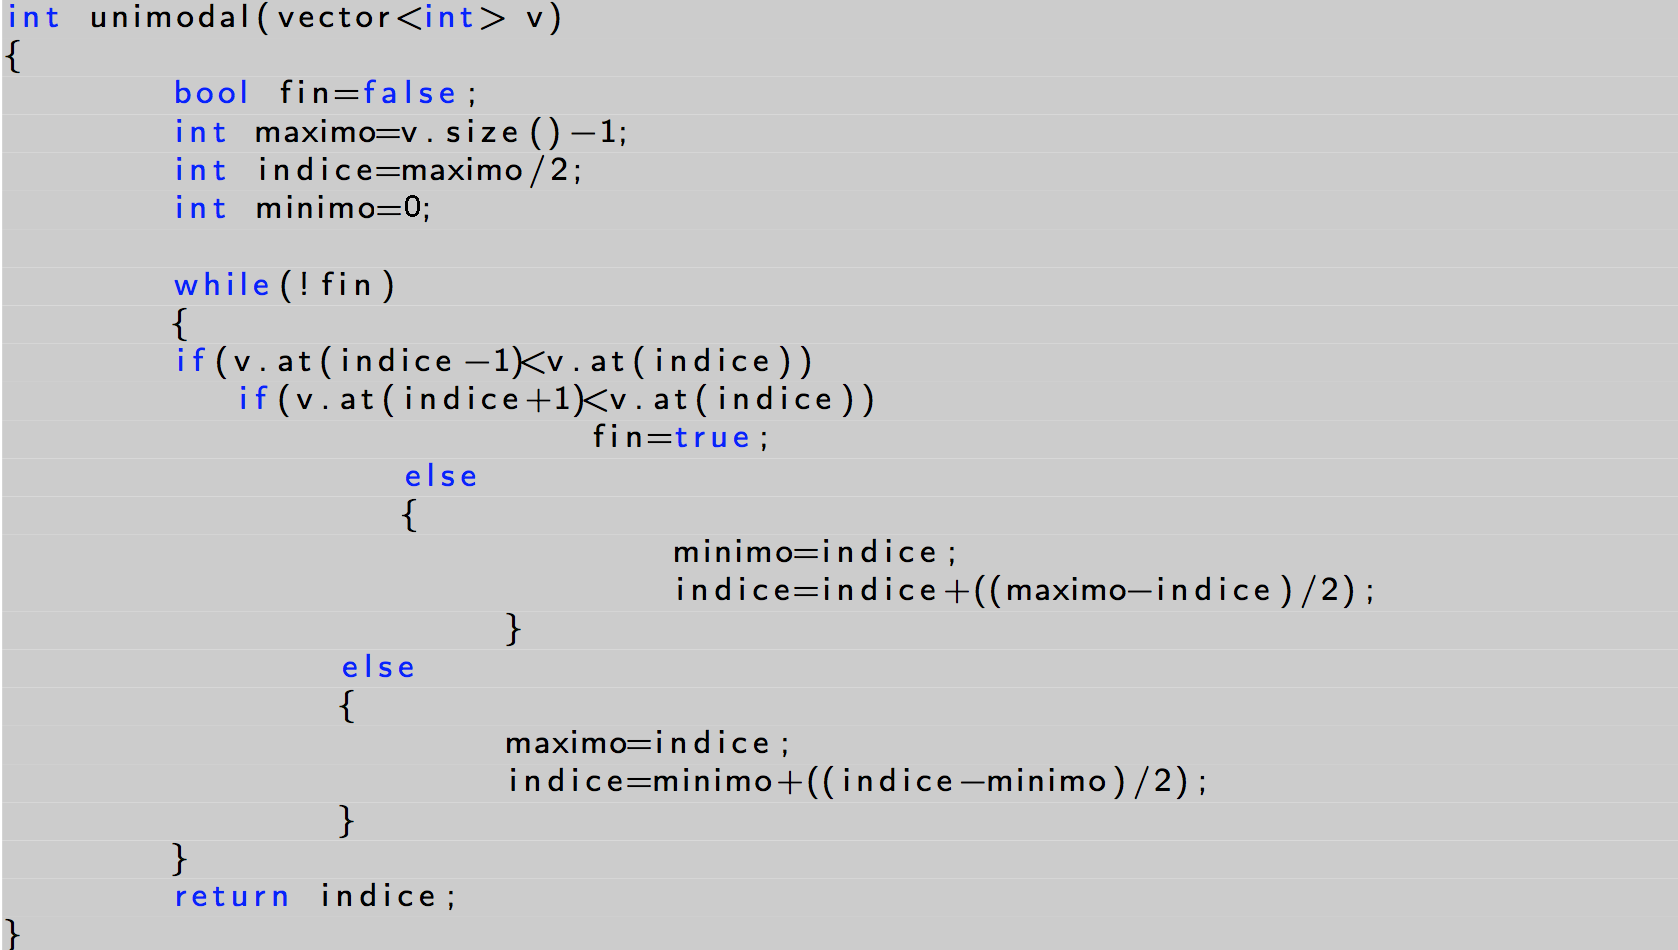
\includegraphics[angle=0,scale=0.35]{img/1.png} 
\label{etiqueta} 
\end{figure}

\end{frame}

\begin{frame}

\begin{figure}[H] 
\centering
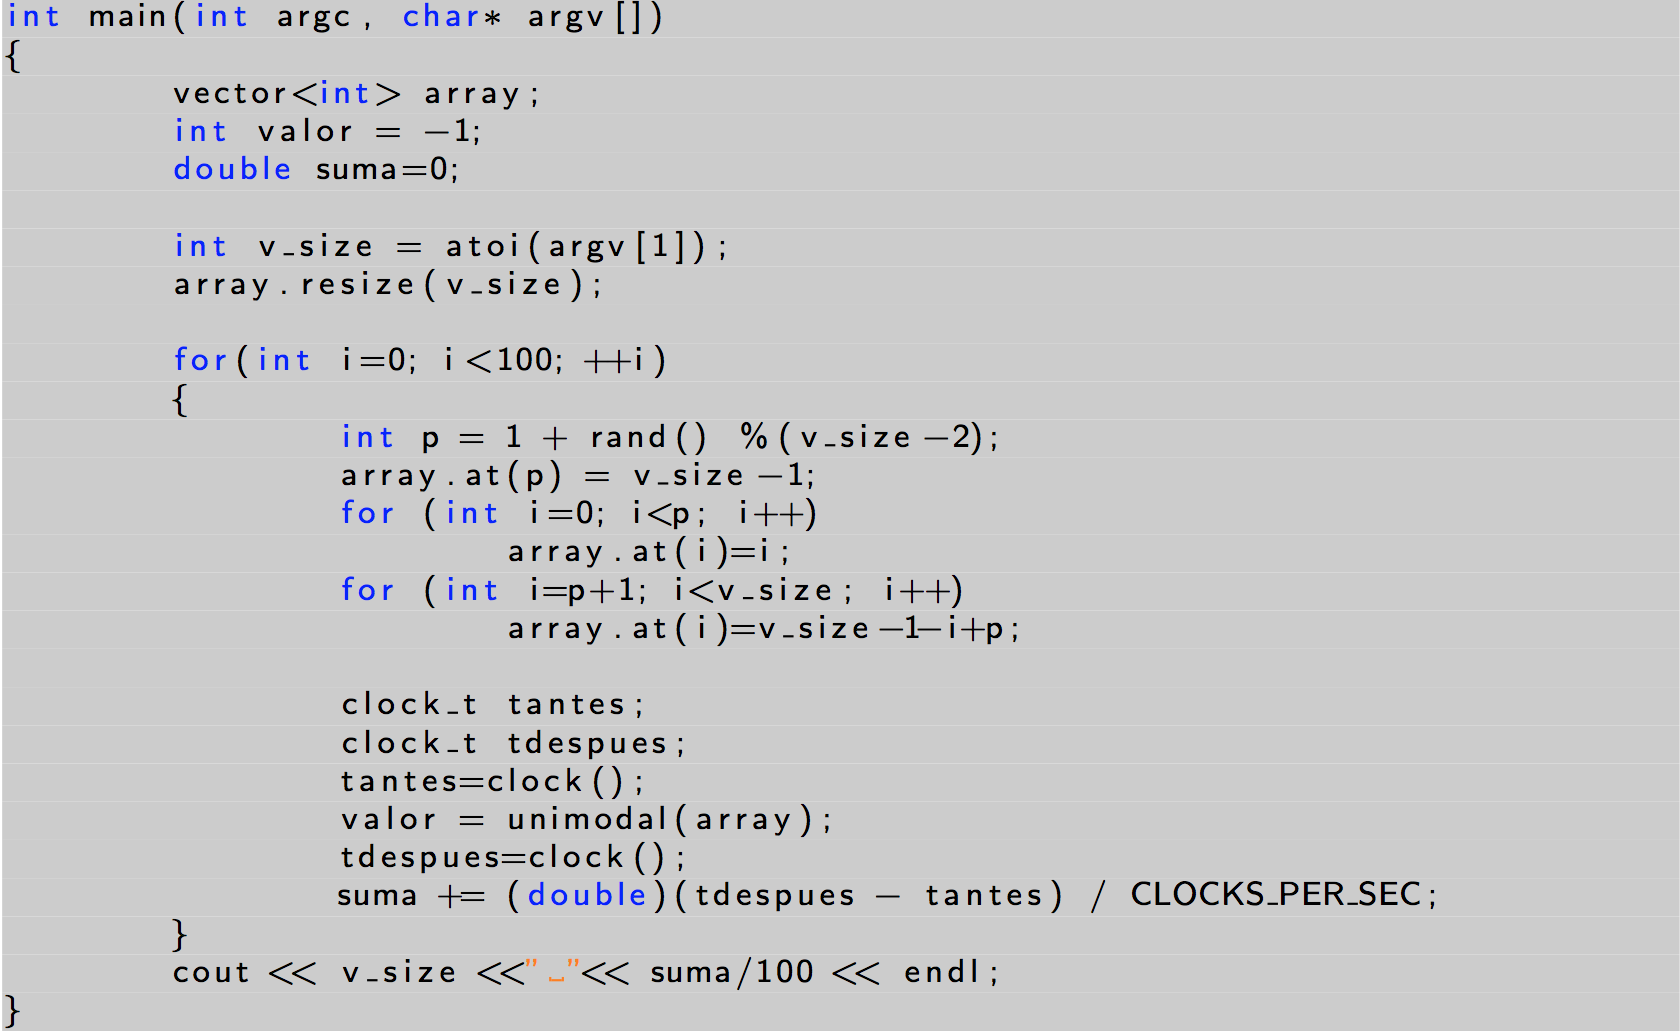
\includegraphics[angle=0,scale=0.35]{img/2.png} 
\label{etiqueta} 
\end{figure}

\end{frame}

\begin{frame}{Código secuencial}
En este caso lo único que se hace es recorrer el vector hasta ver que empieza a ser decreciente.

\vspace{5mm} %5mm vertical space

En el peor caso puede empezar a ser decreciente en el penúltimo elemento por lo que habría que recorrer todo el vector, de manera que la eficiencia de este algoritmo es O(n).
\end{frame}

\begin{frame}

\begin{figure}[H] 
\centering
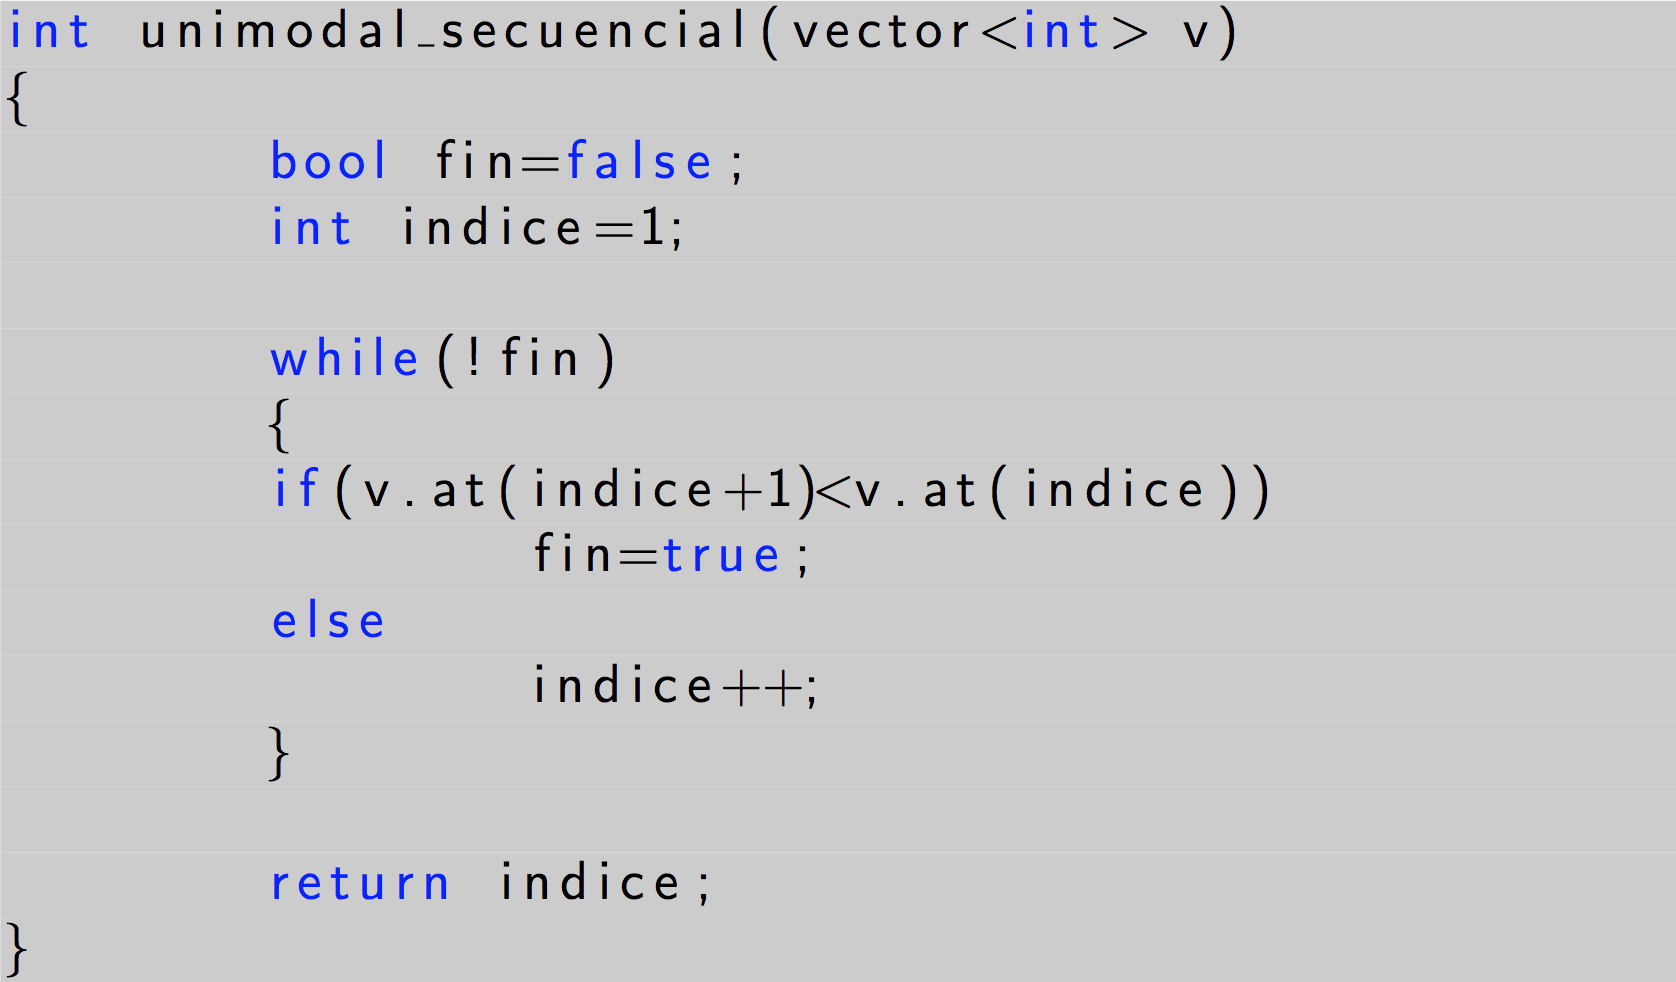
\includegraphics[angle=0,scale=0.35]{img/3.png} 
\label{etiqueta} 
\end{figure}

\end{frame}

\begin{frame}

\begin{figure}[H] 
\centering
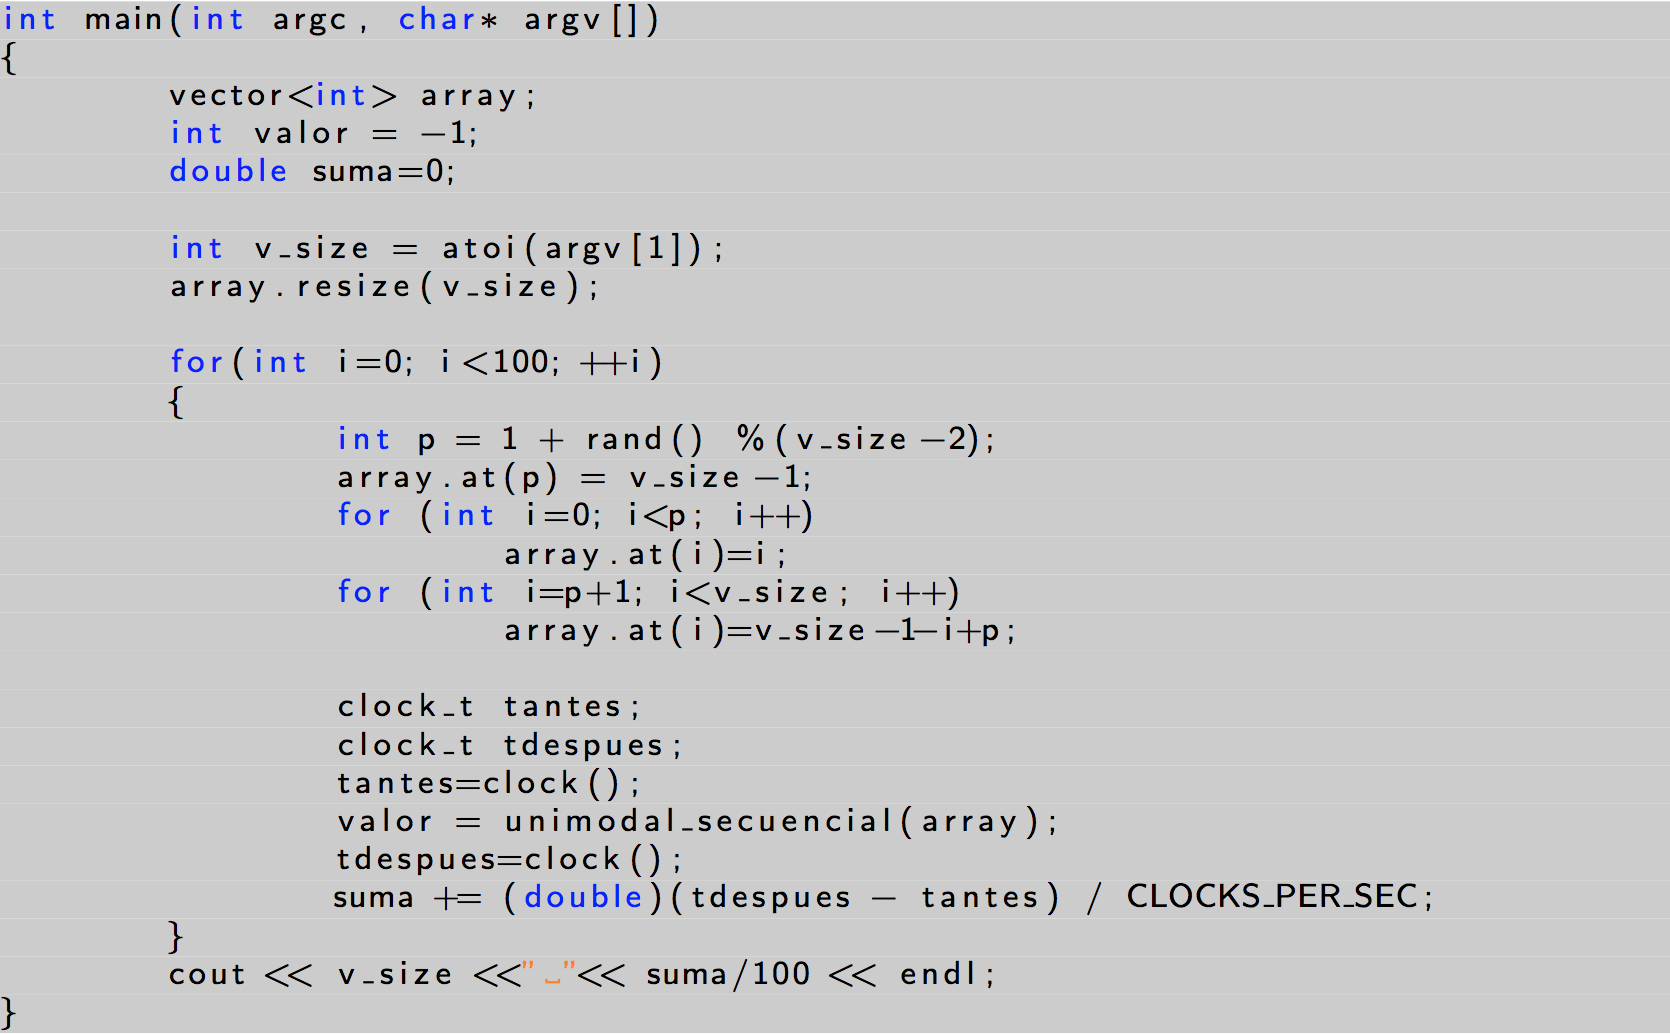
\includegraphics[angle=0,scale=0.35]{img/4.png} 
\label{etiqueta} 
\end{figure}

\end{frame}

\begin{frame}{Eficiencia en el caso secuencial}

\begin{figure}[H] 
\centering
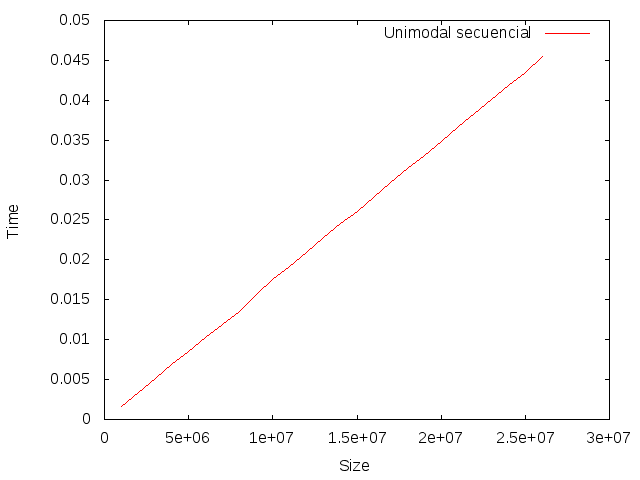
\includegraphics[angle=0,scale=0.4]{img/Eficiencia_sec.png} 
\caption{Pie de imagen} 
\label{etiqueta} 
\end{figure}

\end{frame}

\begin{frame}{Eficiencia en el caso Divide y Vencerás}

\begin{figure}[H] 
\centering
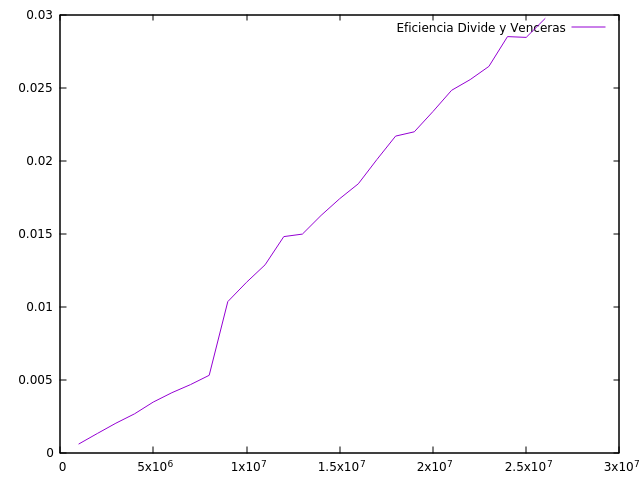
\includegraphics[angle=0,scale=0.5]{img/Eficiencia_dyv.png} 
\label{etiqueta} 
\end{figure}

\end{frame}

\begin{frame}{Eficiencia en el caso Divide y Vencerás}

\begin{figure}[H] 
\centering
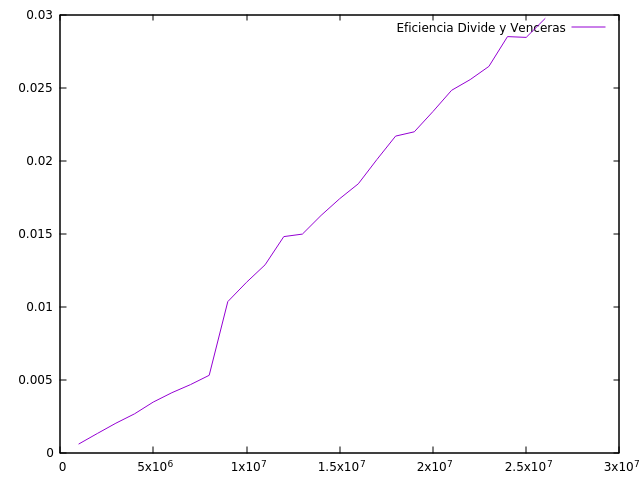
\includegraphics[angle=0,scale=0.5]{img/Eficiencia_dyv.png} 
\label{etiqueta} 
\end{figure}

\end{frame}

\begin{frame}{Ajuste híbrido en el caso secuencial}

\begin{figure}[H] 
\centering
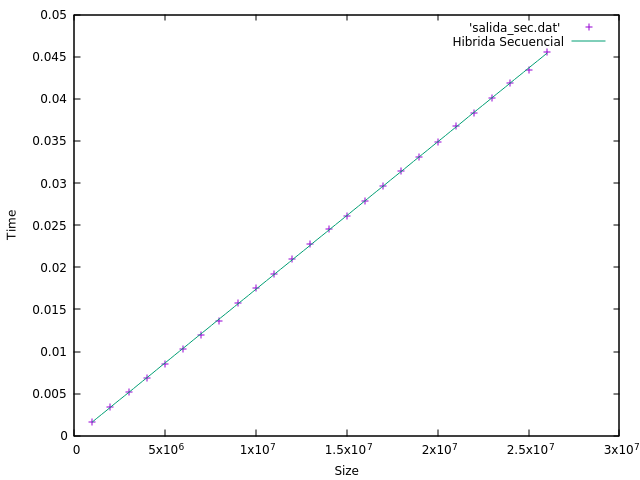
\includegraphics[angle=0,scale=0.5]{img/AjusteHibridoSec.png} 
\caption{Pie de imagen} 
\end{figure}

\end{frame}

\begin{frame}{Ajuste híbrido en el caso Divide y Vencerás}

\begin{figure}[H] 
\centering
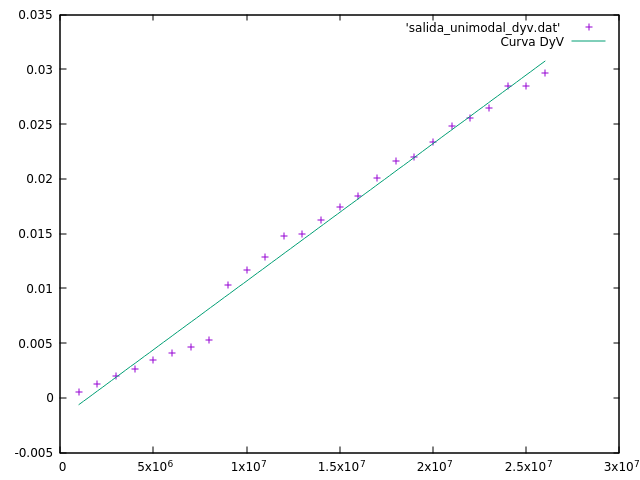
\includegraphics[angle=0,scale=0.5]{img/AjusteHibridoDyV.png} 
\label{etiqueta} 
\end{figure}

\end{frame}

\begin{frame}{Conclusión}

\end{frame}

\end{document}
